\documentclass{article}

\usepackage{qa}

\begin{document}
\customtitle{Homework 5}
\customauthor{Hamza Kamal}
\customdate{\today}

\qna {
     1. Consider the logic gate circuit shown below (5 points) \\
     \begin{figure}[H]
          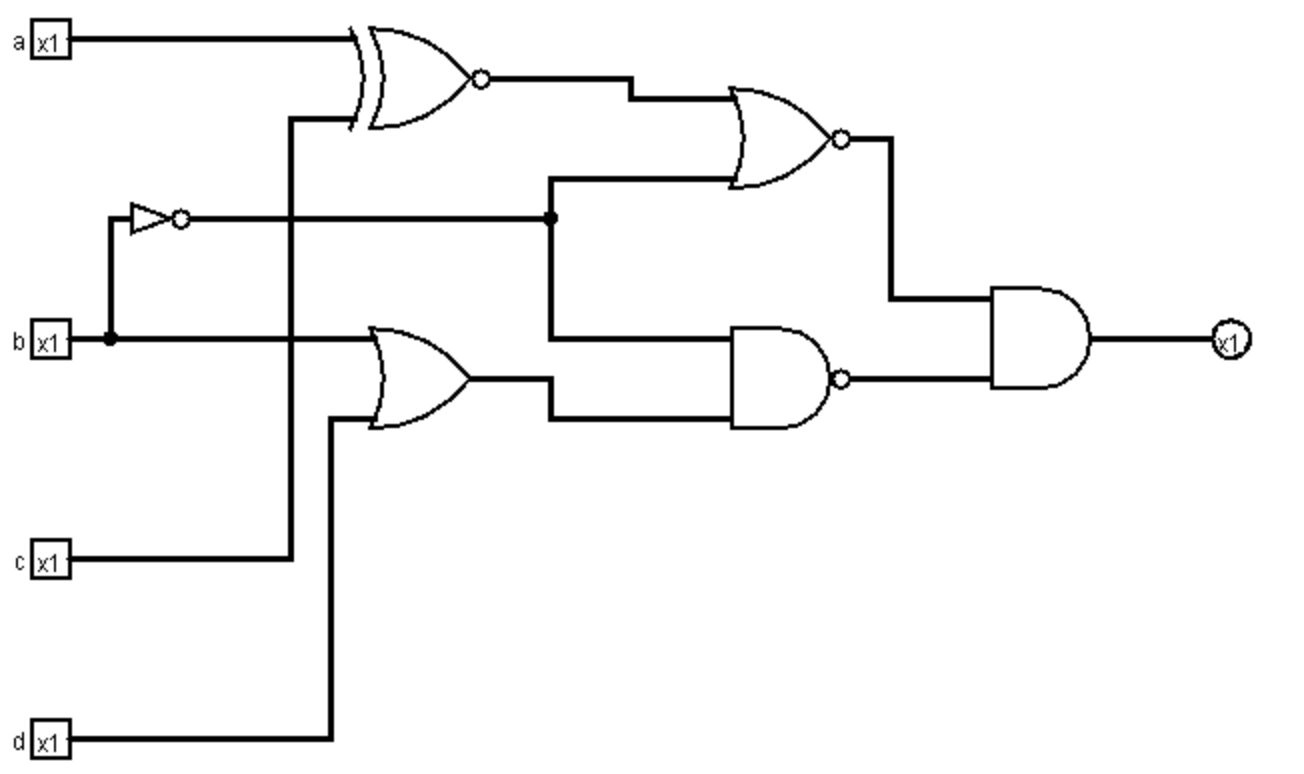
\includegraphics[width=\textwidth]{./img/circuit.png} 
     \end{figure}
     a. (2 points) Derive a Boolean equation for the output X. You don't need to simplify this equation, but feel free to try! \\
} {
     The first gate, which is an XNOR gate with the inputs \(a\) and \(c\), gives us: \\
     \(\neg(a \oplus c)\) \\
     \linebreak
     The second gate is an OR gate with inputs \(b\) and \(d\), which gives us: \\
     \(b \lor d\) \\
     \linebreak
     The third gate is a NOR gate with the inputs \(\neg(a \oplus c)\) and \(\neg b\), which gives us: \\
     \(\overline{\neg(a \oplus c) \lor \neg b}\) \\
     \linebreak
     The fourth gate is a NAND gate with the inputs \(\neg b\) and \(b \lor d\), which gives us: \\
     \(\overline{(\neg b) \land (b \lor d)}\) \\
     \linebreak
     The fifth gate is an AND gate with the inputs \(\overline{\neg(a \oplus c) \lor \neg b}\) and \(\overline{(\neg b) \land (b \lor d)}\), which gives us the final equation: \\
     \(\overline{\neg(a \oplus c) \lor \neg b} \land \overline{(\neg b) \land (b \lor d)}\)
}
\qna {
     b. (3 points) Draw a truth table for the circuit. \\
} {
     Truth Table: \\
     \begin{tabular}{|c | c | c | c | c|}
          \hline
          a & b & c & d & x \\
          \hline
          0 & 0 & 0 & 0 & 0 \\
          \hline
          0 & 0 & 0 & 1 & 0 \\
          \hline
          0 & 0 & 1 & 0 & 0 \\
          \hline
          0 & 0 & 1 & 1 & 0 \\
          \hline
          0 & 1 & 0 & 0 & 1 \\
          \hline
          0 & 1 & 0 & 1 & 1 \\
          \hline
          0 & 1 & 1 & 0 & 1 \\
          \hline
          0 & 1 & 1 & 1 & 1 \\
          \hline
          1 & 0 & 0 & 0 & 0 \\
          \hline
          1 & 0 & 0 & 1 & 0 \\
          \hline
          1 & 0 & 1 & 0 & 0 \\
          \hline
          1 & 0 & 1 & 1 & 0 \\
          \hline
          1 & 1 & 0 & 0 & 1 \\
          \hline
          1 & 1 & 0 & 1 & 1 \\
          \hline
          1 & 1 & 1 & 0 & 1 \\
          \hline
          1 & 1 & 1 & 1 & 1 \\
          \hline
     \end{tabular}
}
\end{document}